\chapter{仿真计算结果}
\label{chapter:results}
在确定了仿真计算模型和相关参数后,接下来就要探索非同步释放对单个神经元和神经元网络的影响。

\section{模型参数}
\label{section:results:parameters}
默认情况下选用表\ref{table:parameters}中的最优参数进行仿真计算。

\section{通过调整模型参数模拟非同步释放的变化}
\label{section:result:modulate-asynchronous-release}
不同类型的类型的神经元能够具有不同的模型参数。
同一种类型的神经元,在不同的环境下也可能具有不同的模型参数。
接下来我们将展示不同参数的变化对突触的最终递质释放的影响。
为了使描述更加清晰,我们将同步释放与非同步释放造成的 IPSC 分别展示。
即,基于式\ref{equation:total-release},我们把 IPSC 分解为 $I_\text{sr}$ 和 $I_\text{ar}$
\begin{align}
I_\text{syn}(t) &= I_\text{sr}(t) + I_\text{ar}(t) \\
I_\text{sr}(t) &= \int_{-\infty}^t e^{-\frac{t - t'}{\tau_\text{GABA}}} w(v - E_\text{GABA})\left( q_\text{sr}(t') + q_\text{s\&a}(t') \right) \dd{t'} \\
I_\text{ar}(t) &= \int_{-\infty}^t e^{-\frac{t - t'}{\tau_\text{GABA}}} w(v - E_\text{GABA})q_\text{ar}(t') \dd{t'}
\end{align}

$\tau_\text{ar}$, $U_\text{ar}$ 和 $X_F / x_0$ 这三个参数直接影响非同步释放,以下将依次展现影响效果。

\subsection{模拟钙离子清除变慢导致的非同步释放增强}
\label{section:result:modulate-with-tau-ar}
对癫痫病人脑组织中的快速发放神经元进行参数拟合后发现,非同步释放的衰减常数为 $\tau_\text{ar} = 8$ ms (见表\ref{table:parameters}),这意味着神经元停止发放后非同步释放减弱速率很快。
前人的研究中发现,表达了 CCK 的神经元中发放停止后非同步释放的衰减速率较慢 \cite{Hefft2005}。
机制上,释放速率的快速降低可能是由于快速发放神经元细胞内包含的 PV 物质导致。
PV 是一种蛋白质,能够使自由钙离子浓度快速下降,导致钙离子感受器快速去激活。
因此 $\tau_\text{ar}$ 在包含 PV 的快速发放神经元中相对较小。
同时,前人的研究也发现钙离子的快速清除能够导致非同步释放减弱 \cite{Jiang2015}。

在试验中,经常使用 EGTA-AM 溶液浸泡来调节细胞内自由钙离子的清除速率。
增加 EGTA-AM 可以提高钙离子的清除 \cite{Otsu2004,Jiang2015}。
这种调控对应于模型中 $\tau_\text{sr}$ 与 $\tau_\text{ar}$ 的改变。
由于两类钙离子感受器具有不同的生物化学性质,所以同一操作对 $\tau_\text{sr}$ 和 $\tau_\text{ar}$ 能造成不同的影响。

我们调节 $\tau_\text{ar}$ 来展示这一参数对同步释放和非同步释放的影响。
将 $\tau_\text{ar}$ 从 $8$ ms 增大到 $30$ ms 能够使 $u_\text{ar}$ 衰减速率明显减缓,这样 $u_\text{ar}$ 就能够在持续发中积累并饱和在一个较高的水平,导致更大的 $I_\text{ar}$ (见图\ref{figure:modulation-of-tau-ar})。
此外,非同步释放增强导致可释放的递质资源 $x$ 变小,间接导致 $I_\text{sr}$ 减小。
这种形式的竞争现象在前人的实验中也有发现 \cite{Otsu2004}。
最终,在发放结束后,非同步释放的电流由于衰减变慢而持续时间更长。

 
\begin{figure}
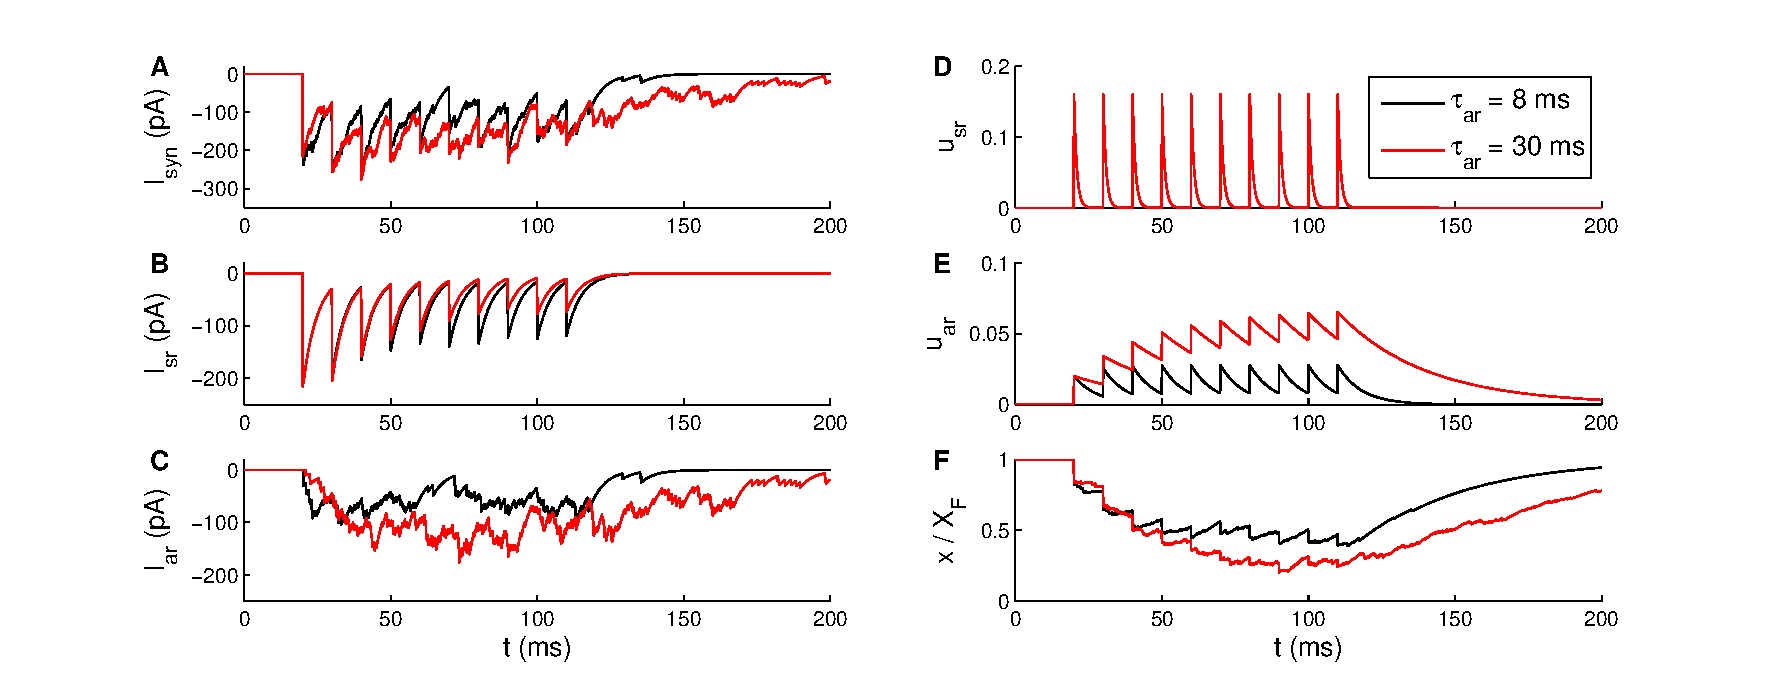
\includegraphics[scale=0.5]{sync-vs-async-ipsc-internals-tau-ar.eps}
\caption{模型中 $\tau_\text{ar}$ 对非同步释放的影响。
仿真计算使用表\ref{table:parameters}中的参数作为默认参数。
$\tau_\text{ar}$ 使用自定义的值,黑线对应 $\tau_\text{ar} = 8$ ms,红线对应 $\tau_\text{ar} = 30$ ms。
神经元发放开始于 $20$ ms,结束于 $110$ ms,发放频率为 $100$ Hz (每次共 $10$ 个动作电位)。
一个量子化释放导致的 IPSC 的高度为 $Ax_0 = 10$ pA。
(A) 总的递质释放导致的 IPSC。
(B) IPSC 中同步释放导致的部分。
(C) IPSC 中非同步释放导致的部分。
(D) 内部状态 $u_\text{sr}$。
(E) 内部状态 $u_\text{ar}$。
(F) 内部状态 $x$ (缩放比例为 $1:X_F$)。}
\label{figure:modulation-of-tau-ar}
\end{figure}


\subsection{模拟神经元动作电位变化导致的非同步释放变化}
\label{section:result:modulate-with-u-ar}
在大鼠的脑组织中发现,癫痫组织细胞的动作电位比正常组织细胞的更高 \cite{Jiang2012}。
理论上更高的动作电位会导致电压依赖的钙离子通道打开更大,使更多的钙离子流入细胞内,进而导致囊泡上的钙离子感受器激活程度更高。
调节动作电位的高度对非同步释放的影响大于同步释放 \cite{Jiang2012}。
流入的钙离子增多对应于模型中 $U_\text{sr}$ 和 $U_\text{ar}$ 的改变。

我们调节 $U_\text{ar}$ 来展示这一参数对同步释放和非同步释放的影响。
将 $U_\text{ar}$ 从 $0.02$ ms $0.06$ 能够使 $u_\text{ar}$ 在每个动作电位后增长更高,由于 $\tau_\text{ar}$ 较小, $u_\text{ar}$ 在很少几个动作电位后会很快饱和。
更高的 $u_\text{ar}$ 导致更大的 $I_\text{ar}$ (见图\ref{figure:modulation-of-u-ar})。
与之前的仿真结果类似,非同步释放增强导致可释放的递质资源 $x$ 变小,间接导致 $I_\text{sr}$ 减小。
 
\begin{figure}
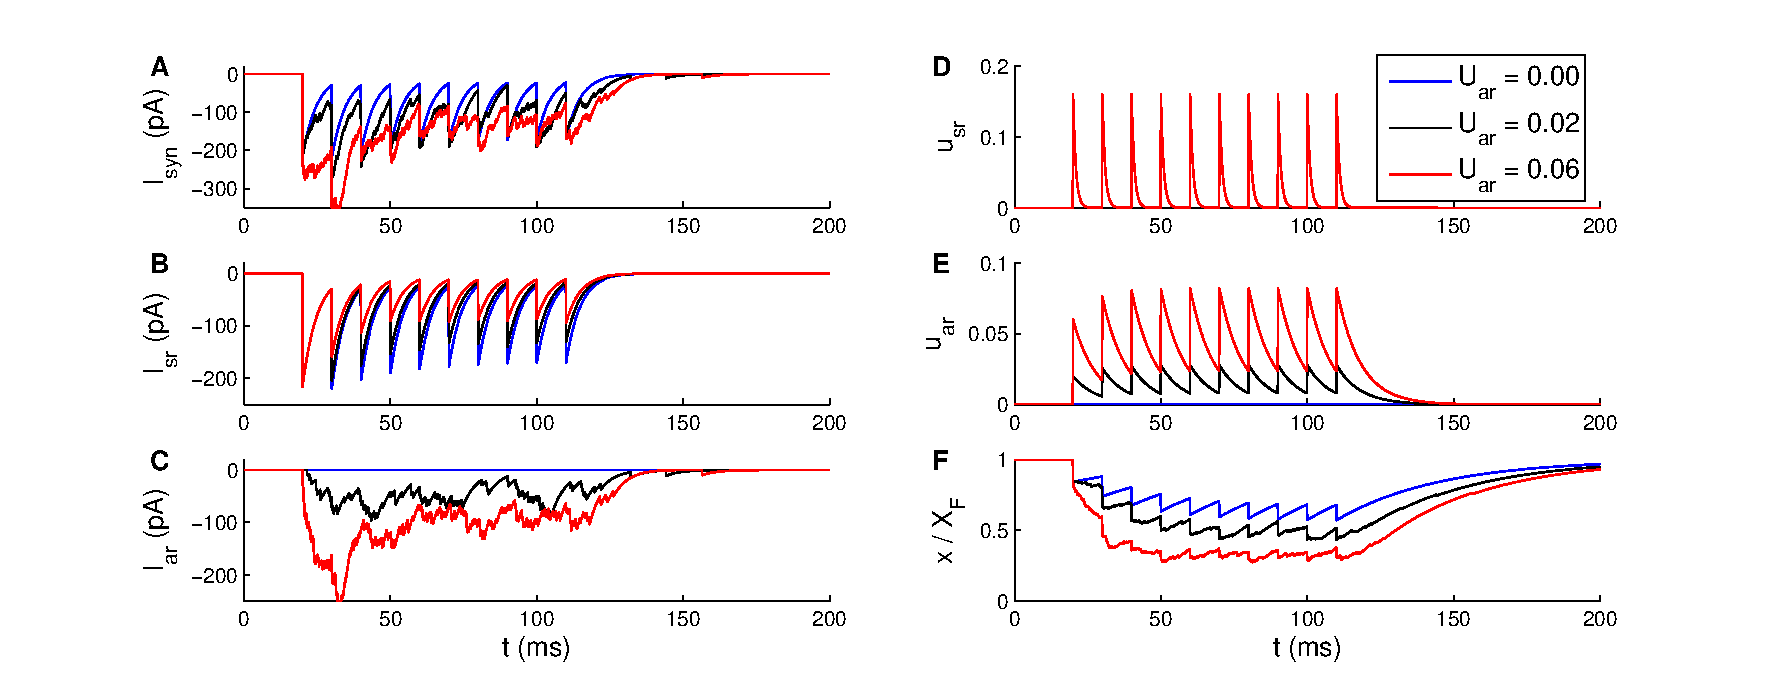
\includegraphics[scale=0.5]{sync-vs-async-ipsc-internals-u-ar.eps}
\caption{模型中 $\tau_\text{ar}$ 对非同步释放的影响。
仿真计算使用表\ref{table:parameters}中的参数作为默认参数。
$U_\text{ar}$ 使用自定义的值,蓝线对应 $U_\text{ar} = 0$,即没有非同步释放,黑线对应 $U_\text{ar} = 0.02$,红线对应 $U_\text{ar} = 0.06$。
神经元发放开始于 $20$ ms,结束于 $110$ ms,发放频率为 $100$ Hz (每次共 $10$ 个动作电位)。
一个量子化释放导致的 IPSC 的高度为 $Ax_0 = 10$ pA。
(A) 总的递质释放导致的 IPSC。
(B) IPSC 中同步释放导致的部分。
(C) IPSC 中非同步释放导致的部分。
(D) 内部状态 $u_\text{sr}$。
(E) 内部状态 $u_\text{ar}$。
(F) 内部状态 $x$ (缩放比例为 $1:X_F$)。}
\label{figure:modulation-of-u-ar}
\end{figure}

\subsection{模拟囊泡相对大小对突触后电流波动的影响}
\label{section:result:modulate-x-0}
我们发现改变 $x_0$ 的相对大小可以影响非同步释放的随机性大小。

假设可释放的递质总量一定,但每个囊泡包含了更少的递质(意味着囊泡数量增多)。
在模型中,保持 $wX_F$ 不变,同时通过减小 $x_0$ 来增加总共可用的囊泡数目 $\frac{X_F}{x_0}$,此处 $w$ 是突触模型中的突触权重(见式\ref{equation:receptor-conductance-general})。

假设在时刻 $t$,剩余递质的比例为 $\xi$。
那么此时共有 $\frac{\xi X_F}{x_0}$ 个囊泡,每一个囊泡在一小段时间内释放的概率都是 $p$,根据二项过程的性质,囊泡释放数量的方差为 $\frac{\xi X_F}{x_0}p(1-p)$。
那么对式\ref{equation:receptor-conductance-general}中的电导 $g$ 造成的方差为
\begin{equation}
\begin{split}
(wx_0)^2 \frac{\xi X_F}{x_0} p (1-p) &= wx_0 (\xi  w  X_F) p (1-p) \\
&= wx_0  c
\end{split}
\label{equation:quantum-effect}
\end{equation}
其中由于 $wX_F$ 保持为常数,故 $c$ 是常数。
因此,对于更大的 $X_F/x_0$, $wx_0$ 会更小,即有递质的随机释放导致的电导的方差更小。
更小的 $wx_0$ 会使非同步释放导致的 IPSC 更光滑(见图)。

\begin{figure}
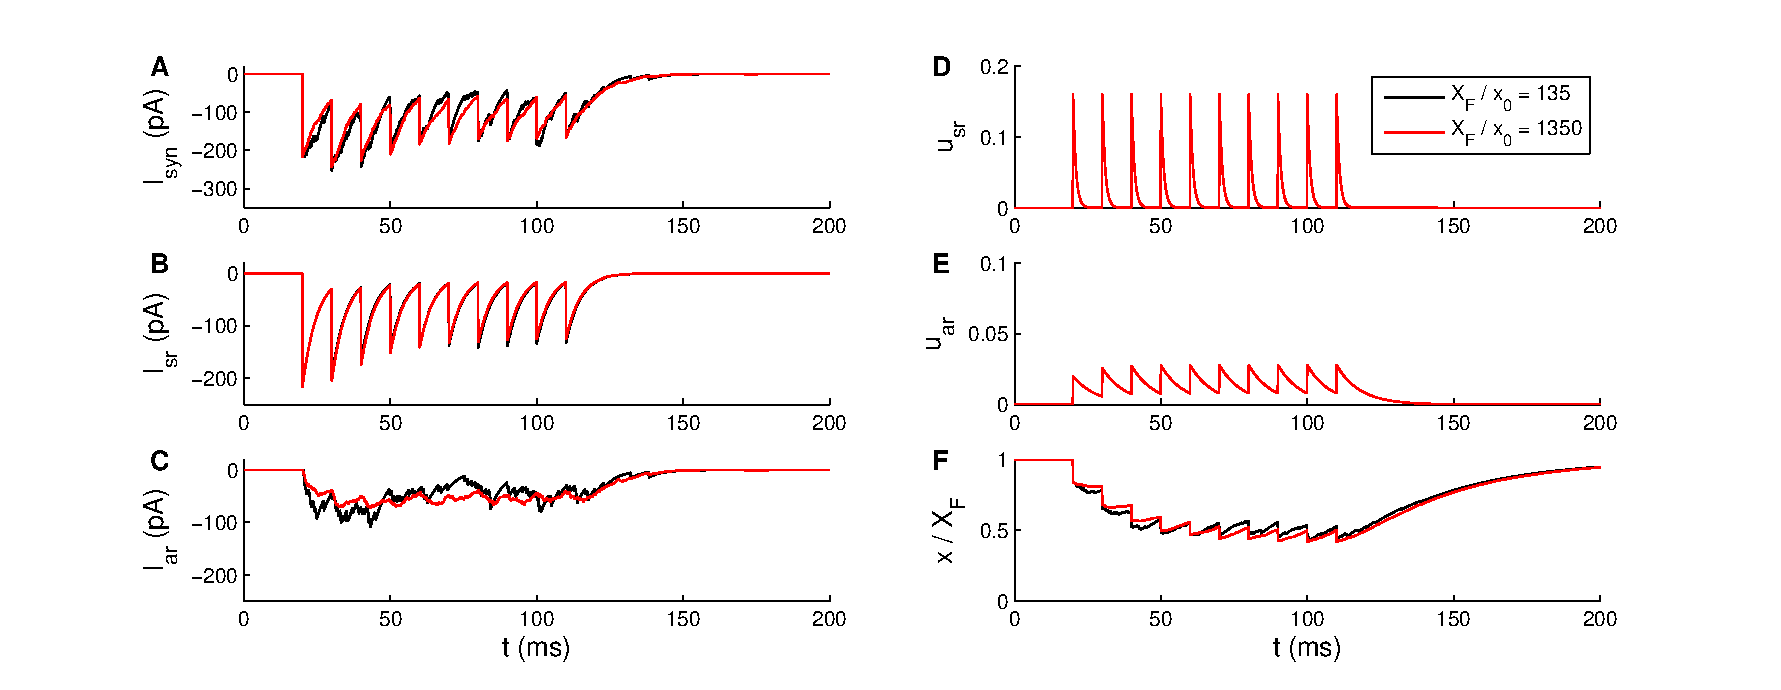
\includegraphics[scale=0.5]{sync-vs-async-ipsc-internals-x-0.eps}
\caption{释放量子大小在模型中对 IPSC 的影响。
黑线设置 $X_F / x_0 = 135$, $Ax_0 = 10$ pA,
红线设置 $X_F / x_0 = 1350$, $Ax_0 = 1$ pA,
其他参数使用表\ref{table:parameters}中的作为默认值。
(A) 总的递质释放导致的 IPSC。
(B) IPSC 中同步释放导致的部分。
(C) IPSC 中非同步释放导致的部分。
(D) 内部状态 $u_\text{sr}$。
(E) 内部状态 $u_\text{ar}$。
(F) 内部状态 $x$ (缩放比例为 $1:X_F$)。
可以明显看出更小的 $X_F/x_0$ 使得 IPSC 更光滑。}
\label{figure:changes-with-x-0} 
\end{figure}


\section{网络仿真计算}
\label{section:resutl:network}
神经元网络仿真计算选择让网络处于同步发放状态,基于此种状态展示非同步递质释放的影响。

神经元网络仿真计算采用 $n = 200$ 个神经元(模型见第\ref{chapter:model}章),突触包含非同步递质释放,突触后递质接收器模型为
\begin{align}
\label{equation:network-receptor-model}
\frac{\dd{g_i\left(t\right)}}{\dd{t}} &= - \frac{g_i\left(t\right)}{\tau_\text{GABA}} + w_i \cdot q_i\left(t - t_\text{delay}\right) \cdot \delta(0) \\
I_\text{syn} &= \sum_i g_i\left(v-E_\text{GABA}\right) \\
I &= - I_\text{syn} + I_\text{ext}
\end{align}
其中 $i$ 为神经元编号,$t_\text{delay} = 1$ ms,$E_\text{GABA} = -70$ mV。
$E(w_i) \approx \frac{w_0}{pn}$, $p$ 为链接概率。

为了使现象更明显,我们放宽了参数的选择范围。
\begin{align}
\label{equation:network-parameters}
\tau_\text{sr} &=  8 \ \text{ms} \\
\Delta U_\text{sr} &= 0.245 \\
\tau_\text{ar} &= 50 \ \text{ms} \\
\Delta U_\text{ar} &= 0.004 \\
\tau_d &= 110 \ \text{ms} \\
x_0/X_F &= 0.01 \\
X_F &= 1
\end{align}


\subsection{非同步释放对网络同步的影响}
\label{section:result:network-synchronization}
非同步释放具有更长的衰减常数,为了展示这一特性的影响,我们采用简化模型(式\ref{equation:ar-release-simplified}),这样递质的释放就变成了没有随机性的过程。
仿真结果显示非同步释放能使网络稳定在同相位状态,而同步释放促使我网络离开同相位状态,进入反相位状态。

模拟参数为 $\tau_\text{GABA} = 5$ ms,$w_0 = 35$ nS, $p = 1$。
网络包含非同步释放时有两种稳定状态——同相位和反相位。
由于非同步释放相对于同步释放较弱,所以同相位的状态转移势垒低于反相位。
网络进入哪一种状态与网络初始状态和背景输入有关(图\ref{figure:network-stability})。

图\ref{figure:network-stability}中每个字图的第一行为每个神经元发放时间的记录,第二行为一个小时间窗口内发放了的神经元占总体的比例,第三行为神经元发放频率的分布,暖色代表高频率。


\begin{figure}
\centering
    \begin{subfigure}{0.45\textwidth}
        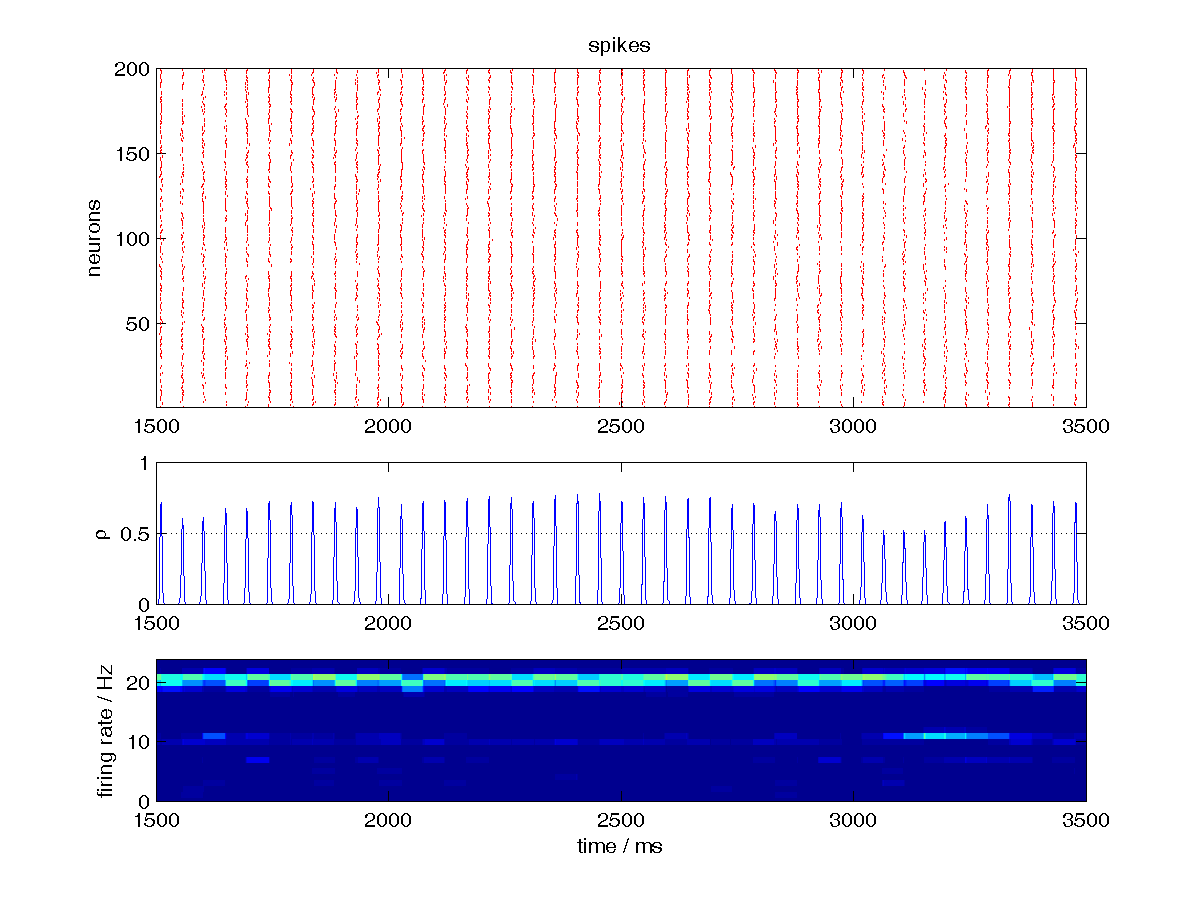
\includegraphics[scale=0.35]{fs-network-mean-in-phase.png}
        \caption{同相位状态。}
    \end{subfigure}
    \begin{subfigure}{0.45\textwidth}
        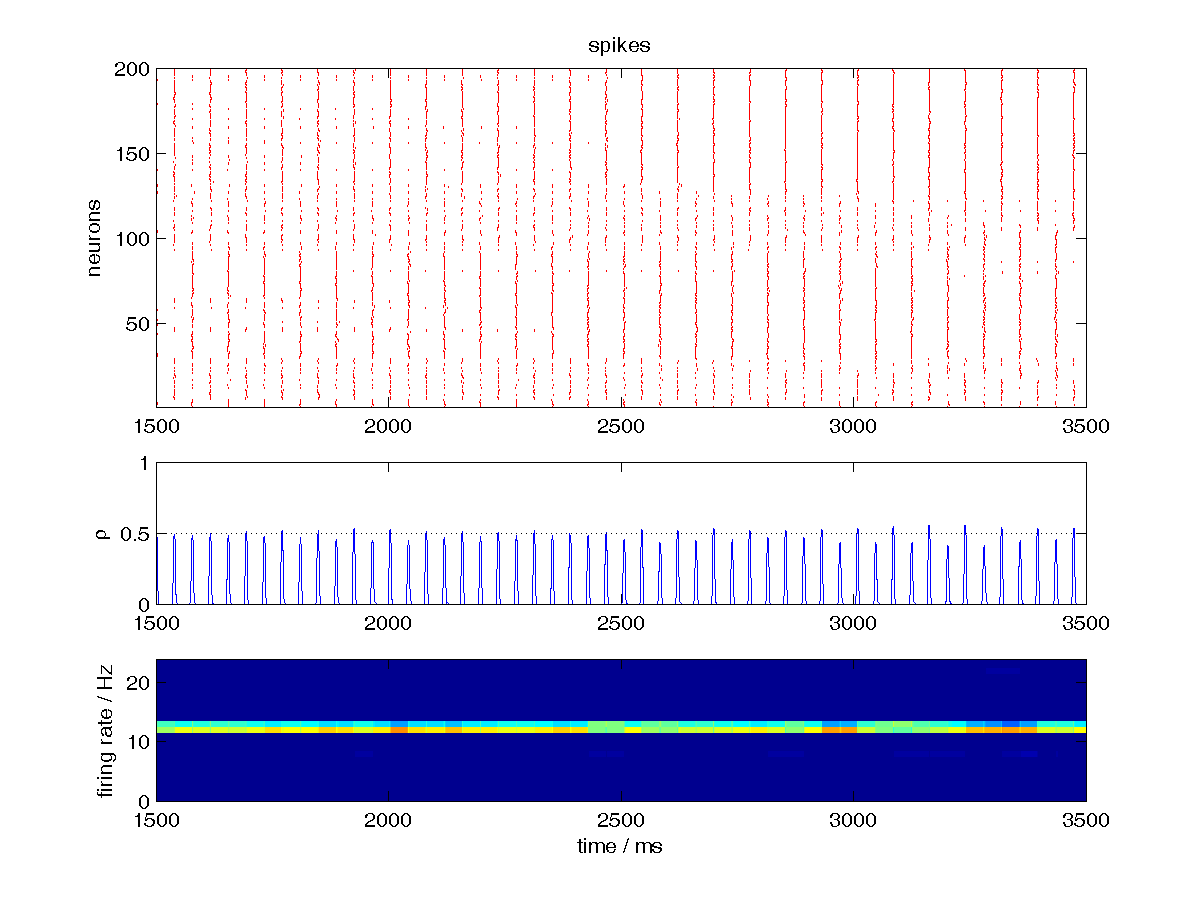
\includegraphics[scale=0.35]{fs-network-mean-anti-phase.png}
        \caption{反相位状态。}
    \end{subfigure}
    \begin{subfigure}{0.45\textwidth}
        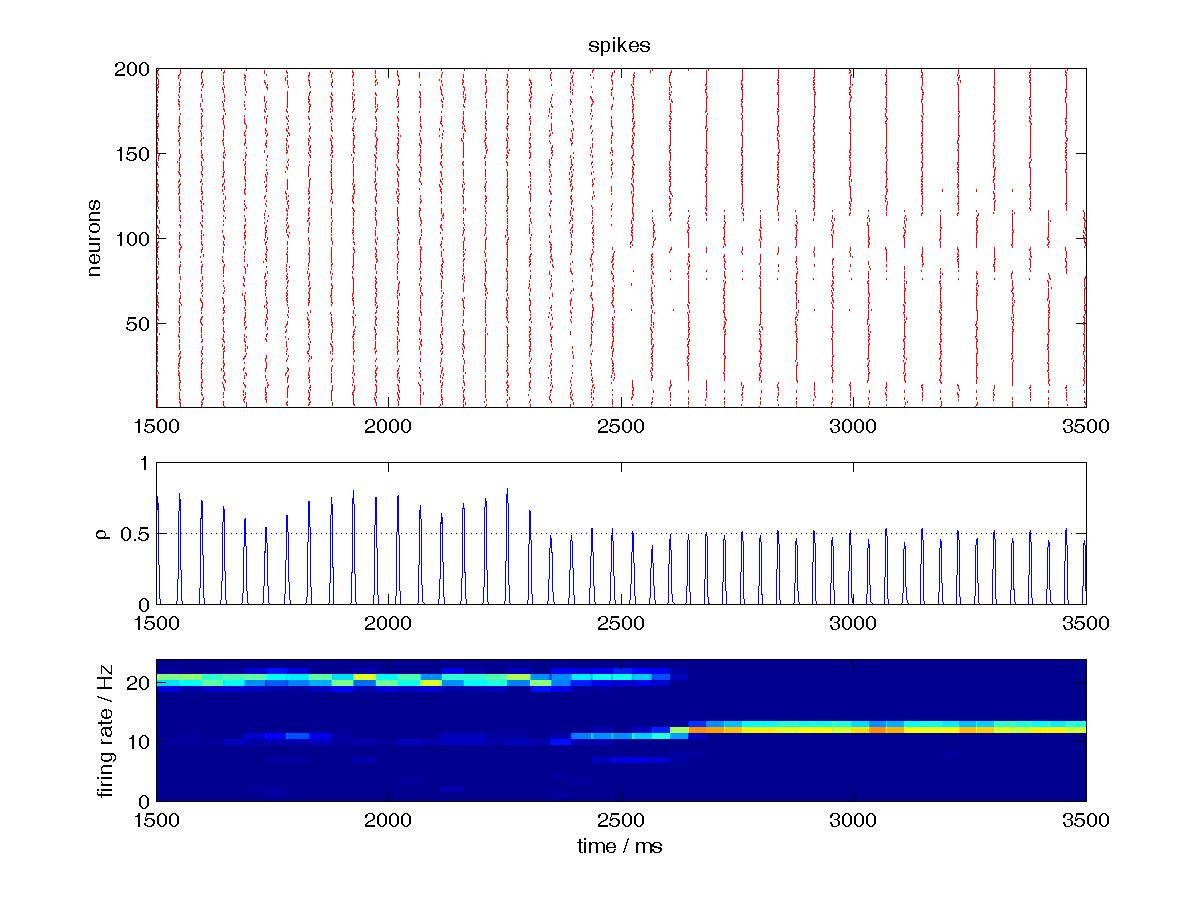
\includegraphics[scale=0.35]{fs-network-mean-transition.png}
        \caption{由同相位转移至反相位。}
    \end{subfigure}
    \begin{subfigure}{0.45\textwidth}
        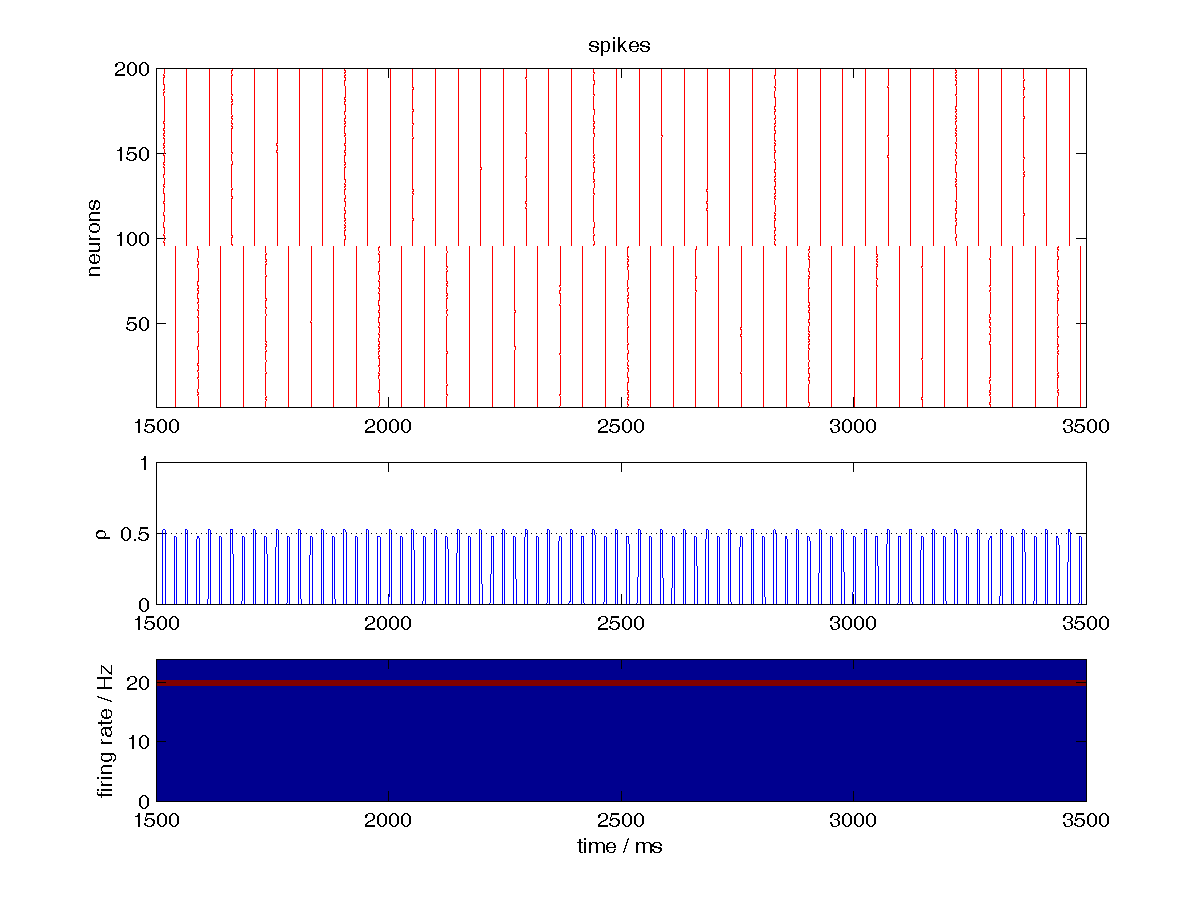
\includegraphics[scale=0.35]{fs-network-mean-block-async.png}
        \caption{没有非同步释放时的网络状态。}
    \end{subfigure}
\caption{网络的两种稳定状态。
背景电流输入为高斯,平均值$I_{\mu} = 80$ pA,$\dd{t} = 0.05$ ms。
非同步释放使用没有随机性的简化模型。
所有仿真计算中神经元和突触使用相同的随机初始状态。
为了使结果更清晰,神经元的编号经过了重新排列。
(a) 背景输入噪声很小 ($I_{\sigma} = 2.4$ pA),网络能够稳定在同相位状态。
(b) 背景噪声增大($I_{\sigma} = 3.2$ pA),网络只能处于反相位状态。
(c) 背景噪声适中($I_{\sigma} = 2.72$ pA),网络能在同相位状态稳定一段时间,之后进入反相位状态。没有观察到网络再回到同相位状态,可能是模拟的时间不够长。
(d) 没有非同步释放时($U_{ar} = 0$),网络进入反相位状态,此时背景噪声很小($I_{\sigma} = 2.4$ pA).}
\label{figure:network-stability}
\end{figure}

\paragraph{使用两个神经元的回路和相位反应曲线进行结果分析}
这里主要分析衰减常数的影响,于是把非同步释放替换为同步释放和衰减较慢的递质感受器。

在两个神经元的回路中,神经元 $\alpha$ 和神经元 $\beta$ 相互连接,没有自连接。背景噪声为高斯,具有相同的平均值和方差。
当两个神经元同步时,在第 $n$ 个周期
\begin{align}
\psi_{\alpha}\left(t\right) &= \left(\phi\left(t\right) + \phi_{\alpha}\left(n\right)\right) \mod 1 \\
\psi_{\beta}\left(t\right) &= \left(\phi\left(t\right) + \phi_{\beta}\left(n\right)\right) \mod 1
\end{align}
其中 $\phi\left(t\right) \in [0,1)$ 为周期函数。

那么两个神经元在第 $n$ 个周期的相位差为
\begin{equation}
\Delta\psi\left(n\right) = \left(\phi_{\alpha}\left(n\right) - \phi_{\beta}\left(n\right)\right) \mod 1
\end{equation}

假设经过一次交互,两个神经元的相位变化不大,且 $f\left(\phi\right)$ 是相位反应曲线,那么 $\alpha$ 的相位延迟为 $f(\Delta\psi\left(n\right))$, $\beta$ 的相位延迟为 $f(1-\Delta\psi\left(n\right))$。

那么在下一个周期,两者的相位差将是
\begin{equation}
\Delta\psi\left(n+1\right) = \left( \Delta\psi\left(n\right) + f(\Delta\psi\left(n\right)) - f(1-\Delta\psi\left(n\right)) \right) \mod 1
\end{equation}

因此,从 $g\left(\Delta\psi\right) = f(\Delta\psi) - f(1-\Delta\psi)$ 中我们可以推测相位差 $\Delta\psi\left(n\right)$ 的稳定性(见图\ref{figure:circuit-anti-phase-in-phase})。

\begin{figure}
    \begin{subfigure}{0.5\textwidth}
        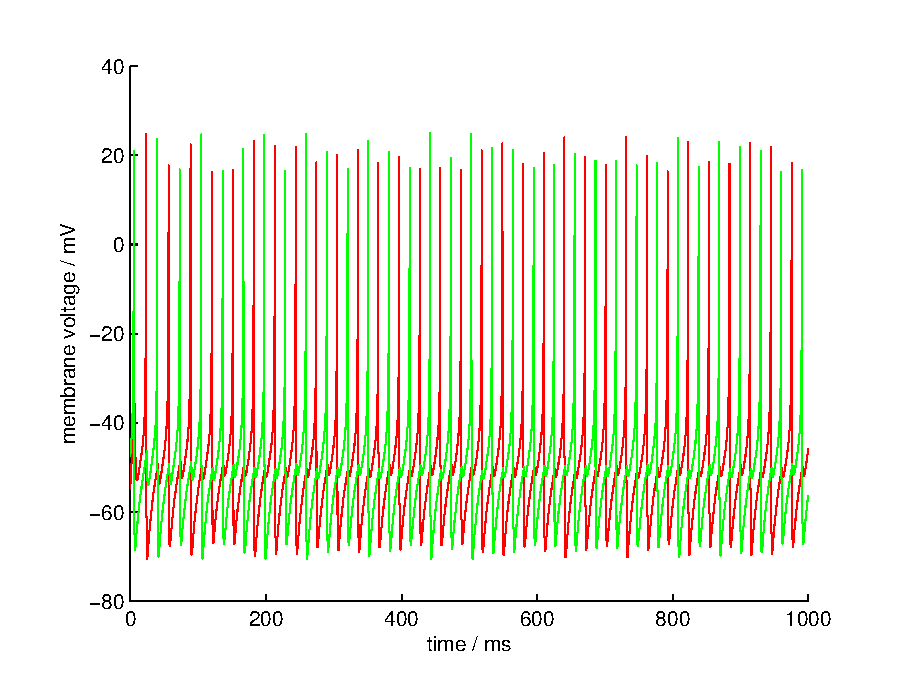
\includegraphics[scale=0.5]{fs-circuit-in-phase-unstable.eps}
        \caption{反相位状态。}
    \end{subfigure}
    \begin{subfigure}{0.5\textwidth}
        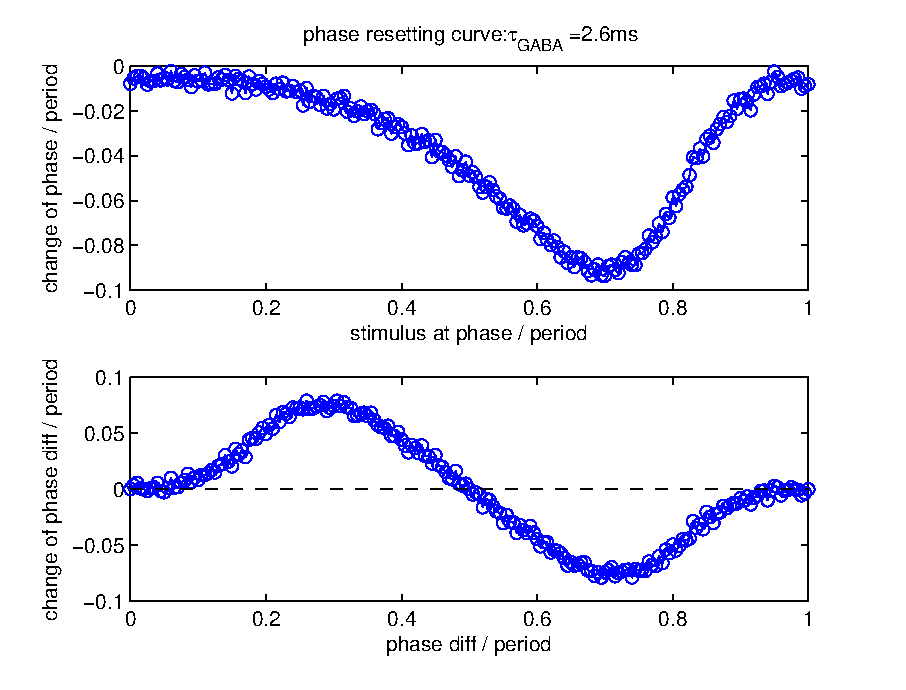
\includegraphics[scale=0.5]{fs-phase-resetting-fast-decay.eps}
        \caption{相位反应曲线。}
    \end{subfigure}
    \begin{subfigure}{0.5\textwidth}
        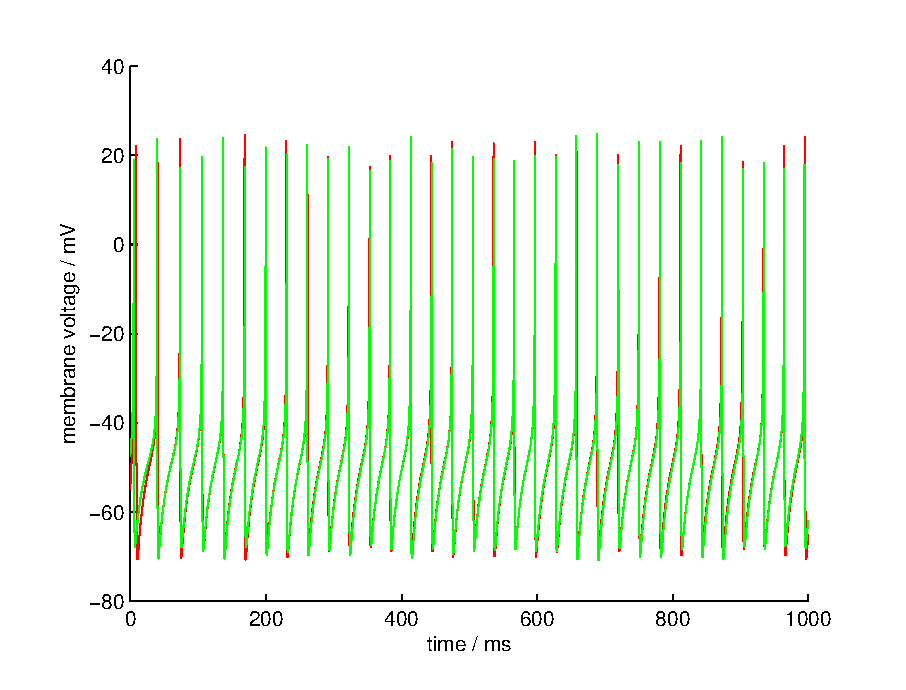
\includegraphics[scale=0.5]{fs-circuit-in-phase-stable.eps}
        \caption{同相位状态。}
    \end{subfigure}
    \begin{subfigure}{0.5\textwidth}
        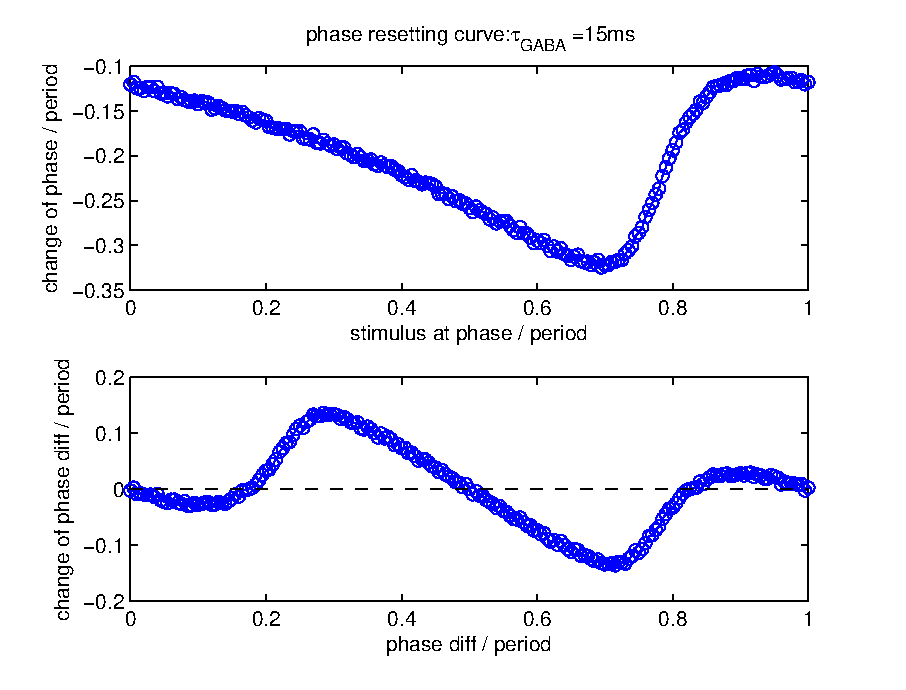
\includegraphics[scale=0.5]{fs-phase-resetting-slow-decay.eps}
        \caption{相位反应曲线。}
    \end{subfigure}
\caption{GABA 衰减常数较小时同相位状态不稳定,较大时同相位状态稳定。
(a) 两个神经元(红色和蓝色)通过 GABA 突触相连。$\tau_\text{GABA} = 2.6$ ms, $w_0 = 40$ nS。背景电流为高斯,平均值为 $I_{\mu} = 100$ pA ,标准差为 $I_{\sigma} = 3$ pA, $\dd{t} = 0.05$ ms。
(b) 对应于(a)中的神经元,上图为相位反应曲线 $f\left(\psi\right)$。下图为 $g\left(\Delta\psi\right)$。可以看出,唯一的稳定点为 $0.5$ 周期。测量相位反应曲线时,$w_{GABA} = 1$ nS。背景电流为常数 $I_{\mu} = 100$ pA, $\dd{t} = 0.005$ ms。
(c) 两个神经元(红色和蓝色)的参数变为 $\tau_\text{GABA} = 15$ ms, $w_0 = 10$ nS。背景电流为高斯,平均值为 $I_{\mu} = 100$ pA ,标准差为 $I_{\sigma} = 3$ pA, $\dd{t} = 0.05$ ms。
(d) 对应于(c),可以看出两个稳定点,分别为 $0$ 和 $0.5$ 周期。测量相位反应曲线时,$w_{GABA} = 1$ nS。背景电流为常数 $I_{\mu} = 100$ pA, $\dd{t} = 0.005$ ms。}
\label{figure:circuit-anti-phase-in-phase}
\end{figure}

非同步递质释放作为一个缓慢衰减的过程,可以使网络更容易稳定在同相位状态。

\subsection{非同步释放对网络发放精确性的影响}
\label{section:result:network-spike-timing}
非同步释放作为一种随机性释放,可能会使网络中神经元发放精确性降低。
基于每个神经元的发放间隔时间统计网络发放的时间精确性。
背景电流 $I_{\mu} = 100$ pA,没有噪声。网络一直处于反相位状态,网络整体发放频率随时间保持稳定。所以方差主要来自神经元之间的差异。

网络采用 $n = 200$ 个神经元,$\tau_\text{GABA} = 5$ ms, $w_0 = 35$ nS, $x_0 / X_F = 0.01$。

仿真计算结果显示更强的非同步释放能导致发放间隔的标准差变大。但影响大小取决于网络连接概率。
虽然突出有随机性,但当网络连接较密时,多个突触对同一个神经元的输入的随机性会相互抵消,所以总体随机性变小,而连接较稀疏时,随机性难以抵消,总体随机性较大(图\ref{figure:spike-timing-precision})。

非同步释放的增强有去同步的效果,但这一效果大小取决于网络连接的疏密程度。对于稠密的网络连接,这一效果可以忽略(图\ref{figure:spike-timing-precision})。

\begin{figure}[H]
    \begin{subfigure}{0.5\textwidth}
        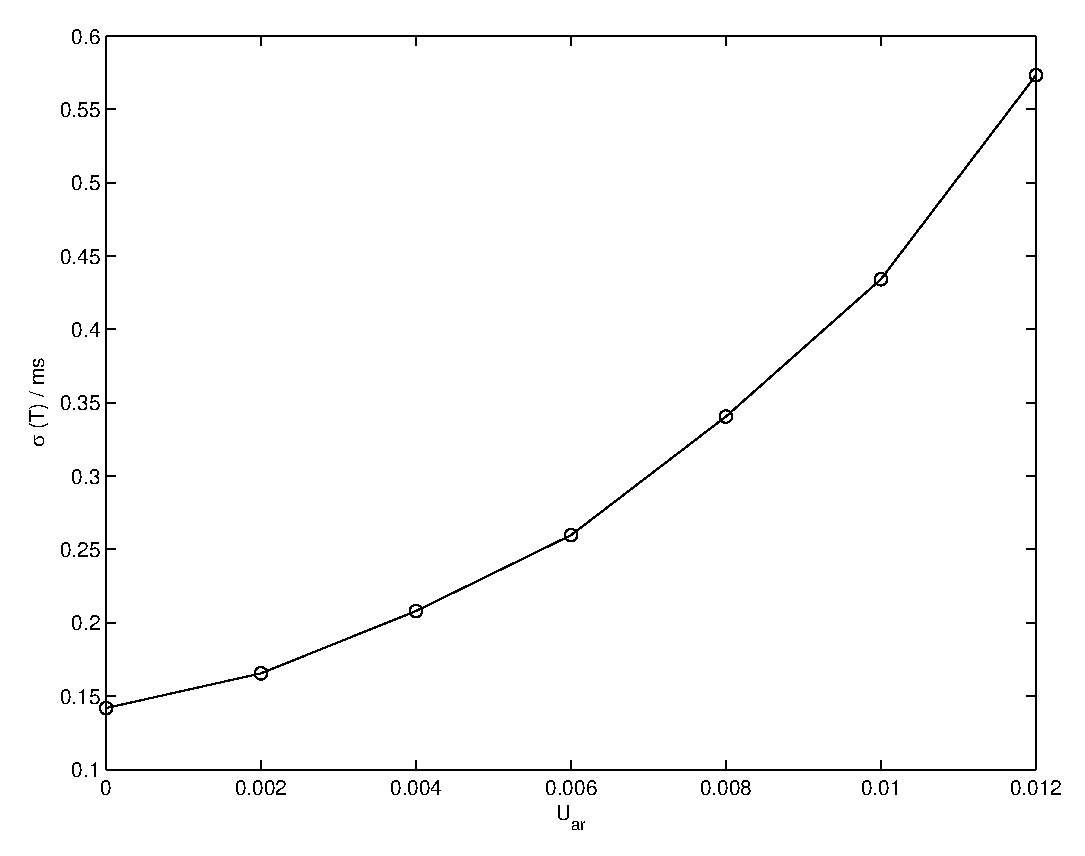
\includegraphics[scale=0.4]{fs-network-spike-timing-std-dense.eps}
        \caption{稠密连接网络中的效果。}
    \end{subfigure}
    \begin{subfigure}{0.5\textwidth}
        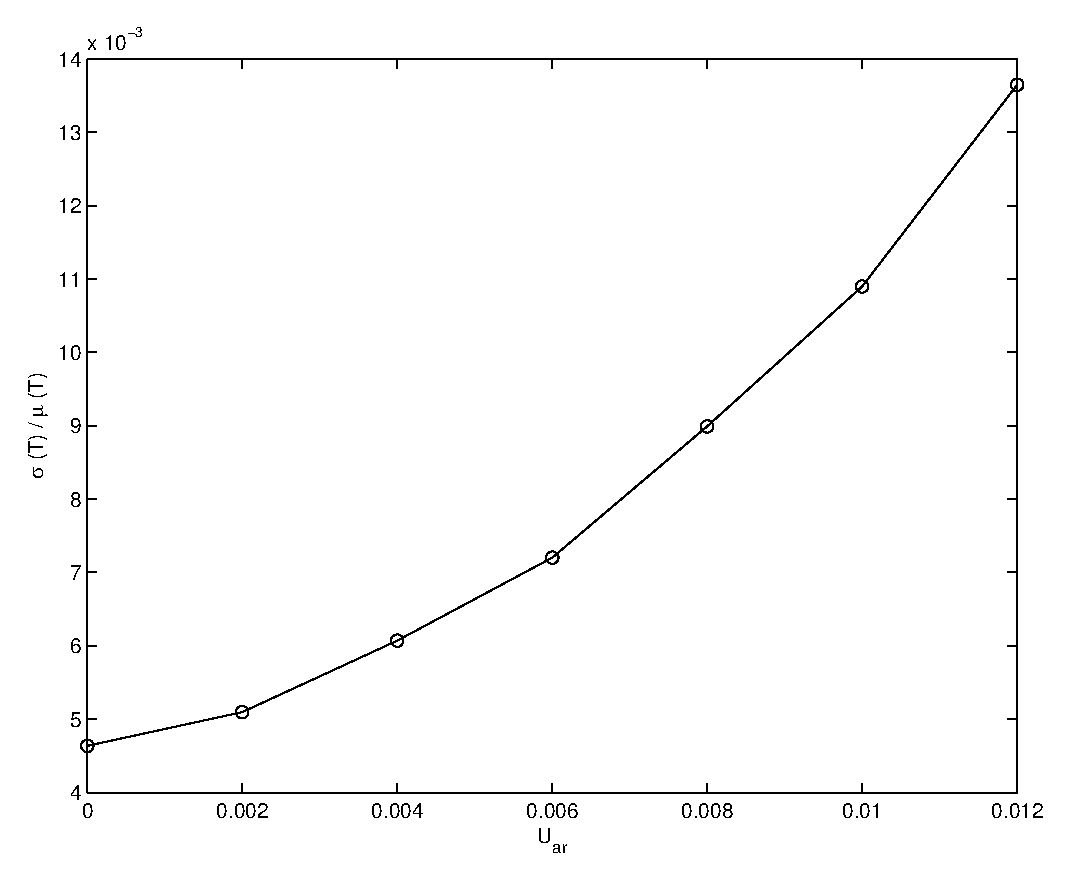
\includegraphics[scale=0.4]{fs-network-spike-timing-relative-dense.eps}
        \caption{稠密连接网络中的相对效果。}
    \end{subfigure}
    \begin{subfigure}{0.5\textwidth}
        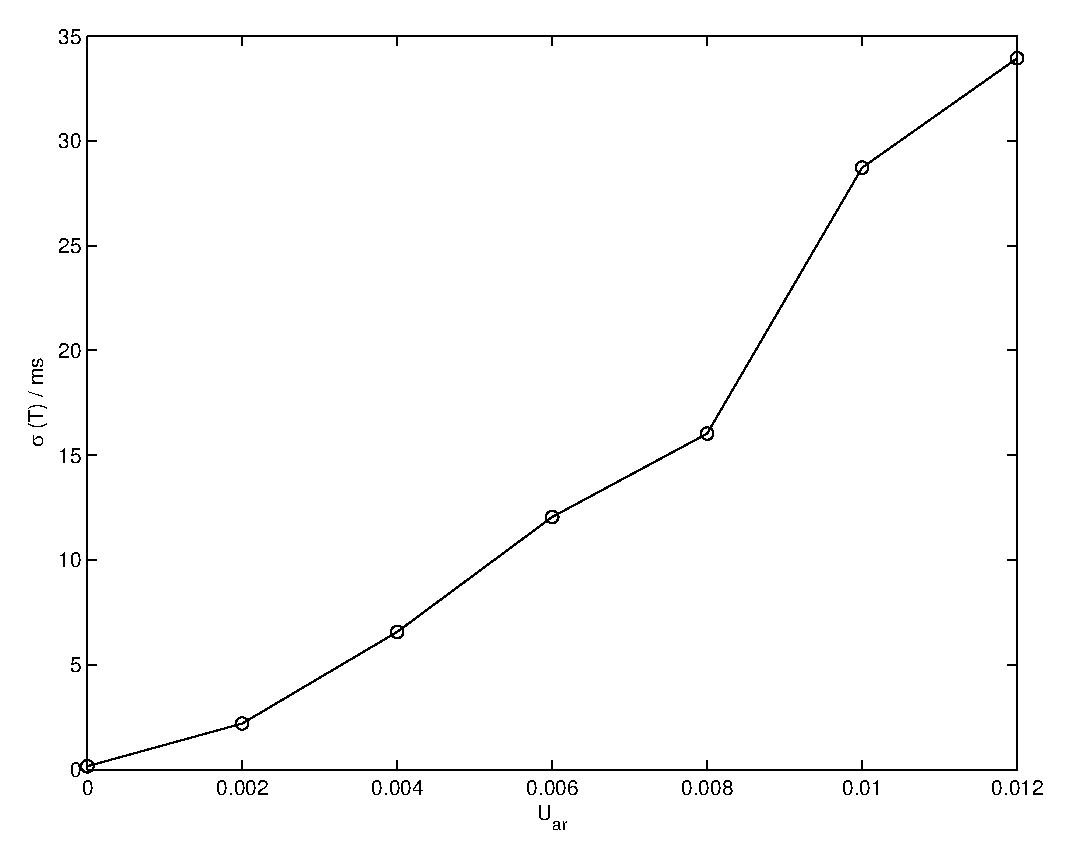
\includegraphics[scale=0.4]{fs-network-spike-timing-std-sparse.eps}
        \caption{稀疏连接网络中的效果。}
    \end{subfigure}
    \begin{subfigure}{0.5\textwidth}
        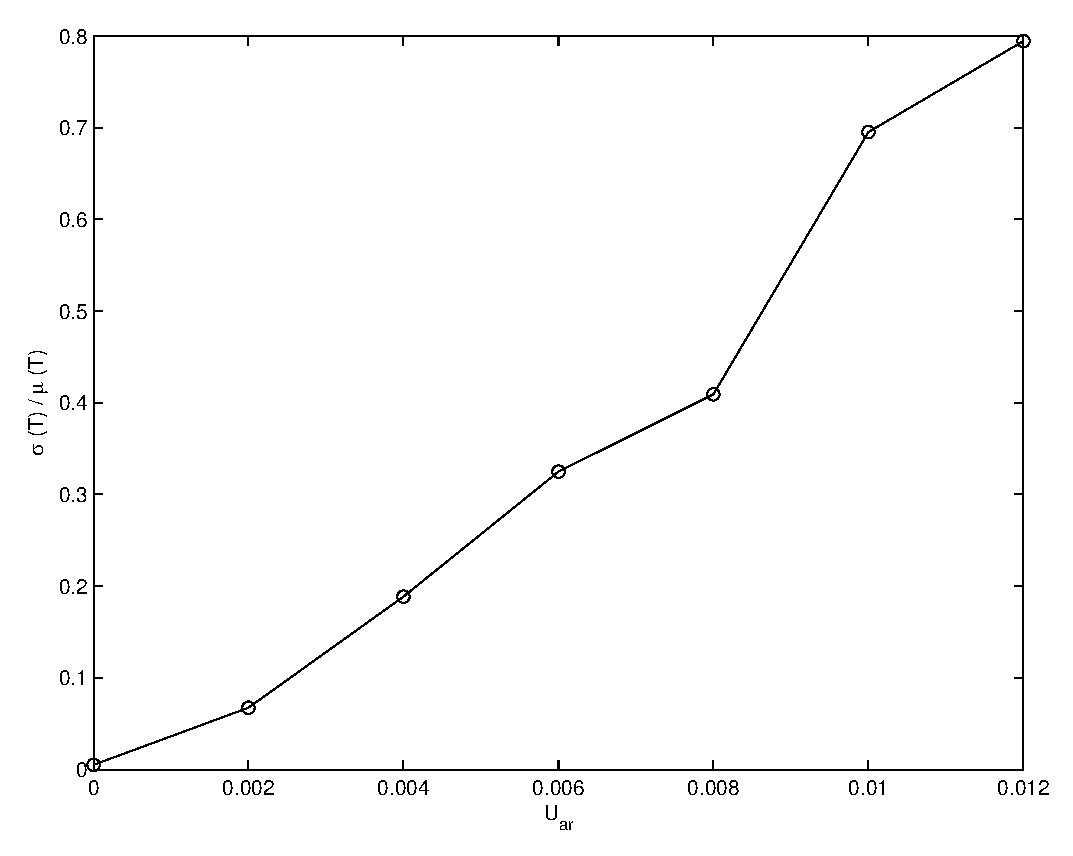
\includegraphics[scale=0.4]{fs-network-spike-timing-relative-sparse.eps}
        \caption{稀疏连接网络中的相对效果。}
    \end{subfigure}
\caption{更强的非同步释放使得神经元发放的时间更不精确。
(a) 发放间隔的标准差 $\sigma(T)$ 随非同步释放的增大(增大 $U_\text{ar}$ )而增大。链接概率为 $p = 1$。
(b) 相对值 $\sigma(T)/\mu(T)$ 也随非同步释放的增大而增大。连接概率为 $p = 1$。
(c) 发放间隔的标准差 $\sigma(T)$ 随非同步释放的增大(增大 $U_\text{ar}$ )而增大。链接概率为 $p = 0.3$。
(d) 相对值 $\sigma(T)/\mu(T)$ 也随非同步释放的增大而增大。连接概率为 $p = 0.3$。
统计使用刺激开始后第 $2$ s 到第 $4$ s 的发放间隔。背景电流为常数 $I_{\mu} = 100$ pA, $\dd{t} = 0.005$ ms。初始状态为随机生成,不同试验中都相同。}
\label{figure:spike-timing-precision}
\end{figure}

\subsection{非同步释放对网络自身的抑制性}
\label{section:result:network-self-inhibition}
网络选用 $n = 200$ 个神经元,$\tau_\text{GABA} = 2.6$ ms,链接概率 $p = 0.3$,$w_0 = 40$ nS。

在突触模型中, IPSC 依赖递质释放率和突触后细胞的细胞膜电位。
在同步发放的网络中,递质释放率与细胞膜膜电位高度相关,所以不能仅仅用 GABA 释放率来度量。
这里我们用网络平均发放频率来度量抑制性效果。

结果显示同步释放的增大(增大 $U_\text{sr}$)对网络抑制效果的影响不如非同步释放的增大(增大 $U_\text{ar}$),网络同步后抑制性主要由非同步释放提供(图\ref{figure:network-recurrent-inhibition})。

\begin{figure}
    \begin{subfigure}{0.5\textwidth}
        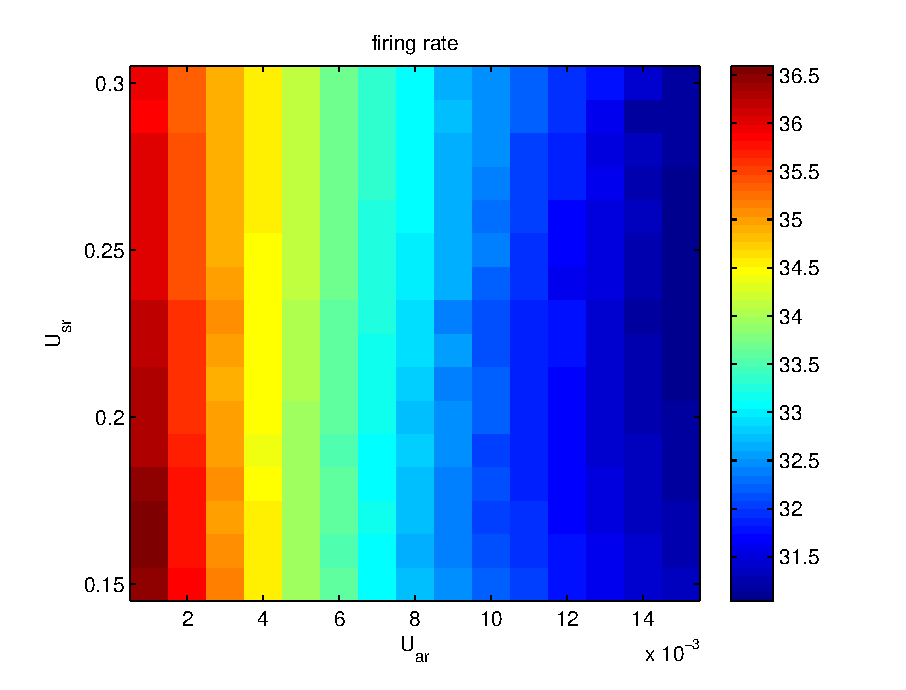
\includegraphics[scale=0.5]{fs-network-stat-u-firing-high-fast.eps}
        \caption{强背景电流。}
    \end{subfigure}
    \begin{subfigure}{0.5\textwidth}
        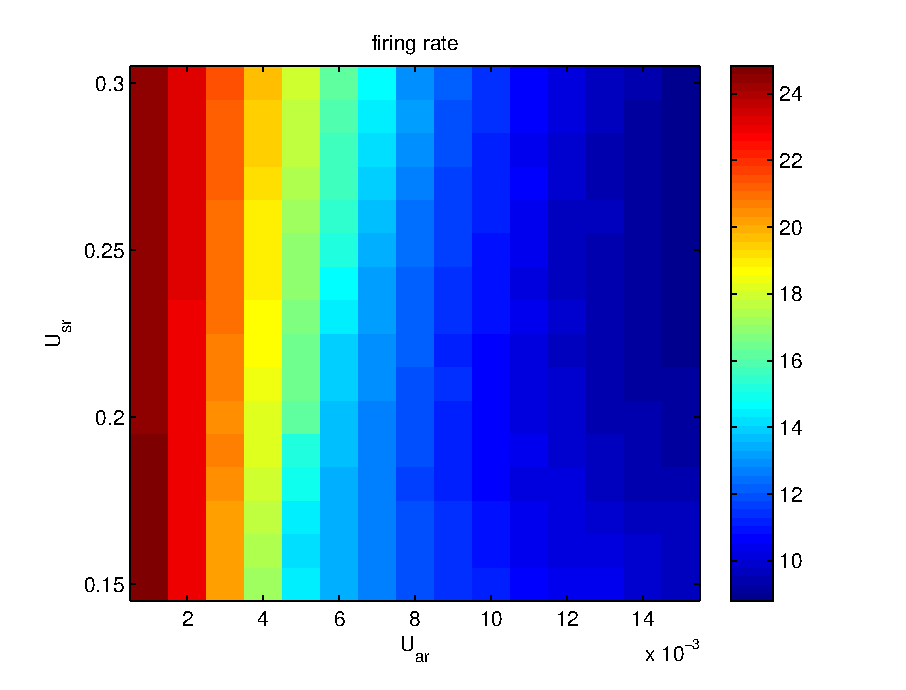
\includegraphics[scale=0.5]{fs-network-stat-u-firing-low-fast.eps}
        \caption{中等背景电流。}
    \end{subfigure}
\caption{同步释放和非同步释放对网络自身 抑制性的影响。
(a) 背景电流为高斯,平均值为 $I_{\mu} = 100$ pA ,标准差为 $I_{\sigma} = 3$ pA。
(b) 背景电流为高斯,平均值为 $I_{\mu} = 80$ pA ,标准差为 $I_{\sigma} = 2.4$ pA。
$\dd{t} = 0.05$ ms。}
\label{figure:network-recurrent-inhibition}
\end{figure}

\paragraph{用单神经元自抑制模型来分析原理}
为了分析网络行为的原理,我们用单个神经元来近似同步发放下的网络。
但个神经元有到自身的突触。
类似地,我们用不同递质接收器衰减常数的模型来分别近似同步释放和非同步释放。

如果固定突触权重,更高的 $\tau_\text{GABA}$ 会导致更高的平均电导。
\begin{equation}
\begin{split}
g_{mean} &= \frac{1}{T} \int_{0}^{T} {g_{GABA}\left(t\right)\dd{t}} \\
& \approx \frac{1}{T} \int_{0}^{\infty} {w \cdot \exp\left(-\frac{t}{\tau_\text{GABA}}\right)\dd{t}} \\
&= \frac{w\cdot \tau_\text{GABA}}{T}
\end{split}
\end{equation}
所以,为了使平均电导相同,我们将把 $w_{GABA}$ 根据 $\tau_\text{GABA}$ 进行归一化。

$Q_{GABA}$ 可以看作是加权求和的结果, $g\left(t\right)$ 则是每一时刻的权重。 $v\left(t\right) - E_{GABA}$ 随时间 $t$ 单调递增,所以更大的 $\tau{GABA}$ 使得权重分布偏向更大的 $v\left(t\right) - E_{GABA}$,这就导致 $Q_{GABA}$ 变大。
由于 $v\left(t\right) - E_{GABA}$ 在一个周期内变化巨大,随意权重的偏移能使 $Q_{GABA}$ 明显变化(见图\ref{figure:fs-neuron-tau-charge})。 

\begin{figure}
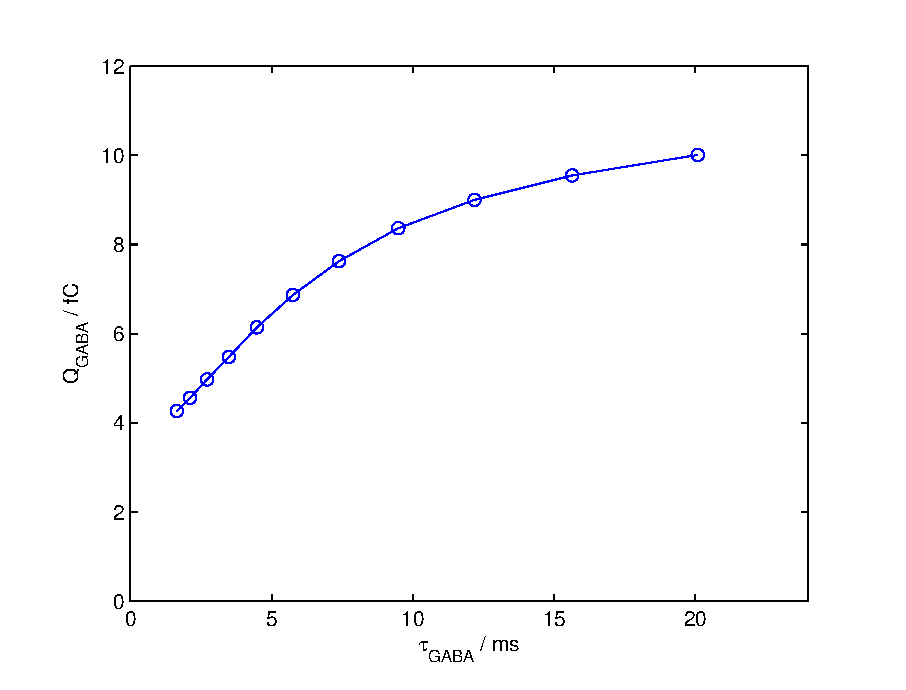
\includegraphics{fs-charge-tau-relation.eps}
\caption{每个周期内的 GABA 电量随 $\tau_\text{GABA}$ 的增大而增大。
突触权重进行了归一化,使得 $w \cdot \tau_\text{GABA} = w_{std} \cdot \tau_{std}$, $w_{std} = 1$ nS, $\tau_{std} = 5$ ms。
背景电流 $I_{\mu} = 100$ pA。
每个 $\tau_\text{GABA}$ 对应的突触权重都非常小,所以不会对发放周期有太大影响。}
\label{figure:fs-neuron-tau-charge}
\end{figure}

统计发放率来比较抑制性也得到了类似的结果(图\ref{figure:fs-neuron-inhibition})。

\begin{figure}
    \begin{subfigure}{0.5\textwidth}
        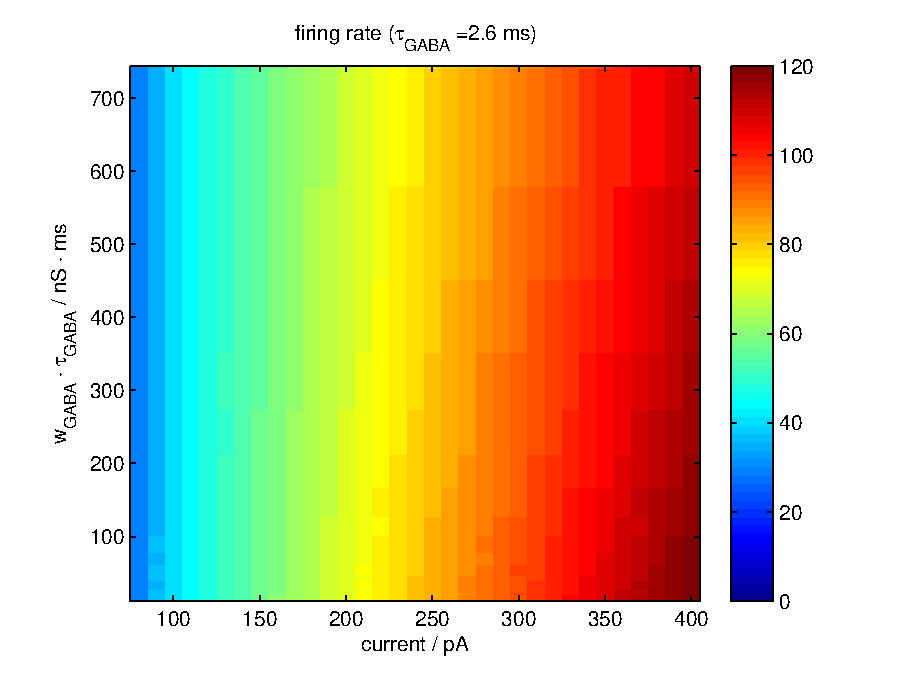
\includegraphics[scale=0.5]{fs-recurrent-input-output-fast-decay-normalized.eps}
        \caption{快速抑制。}
    \end{subfigure}
    \begin{subfigure}{0.5\textwidth}
        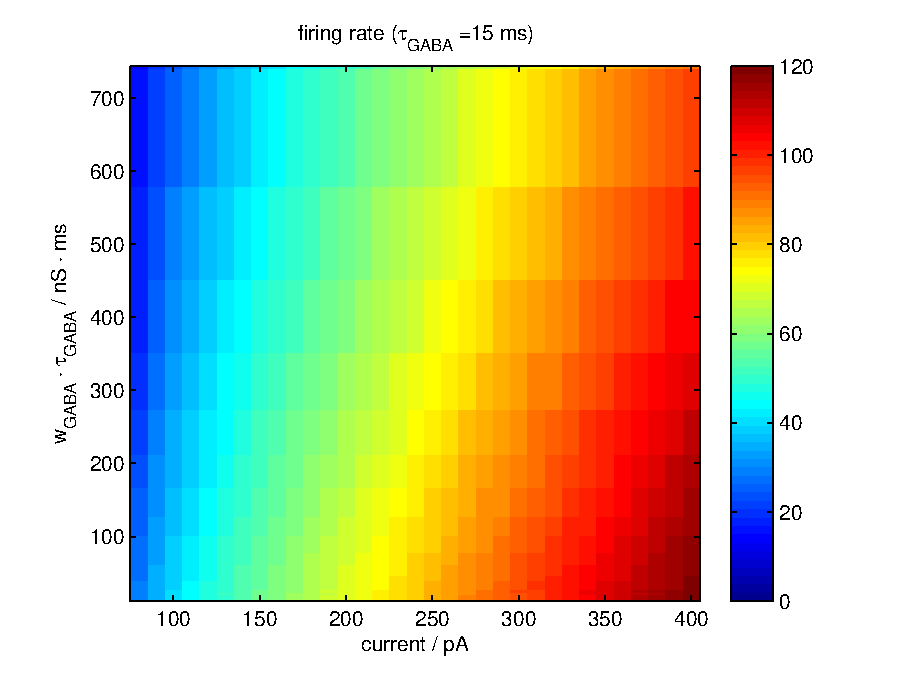
\includegraphics[scale=0.5]{fs-recurrent-input-output-slow-decay-normalized.eps}
        \caption{慢速抑制。}
    \end{subfigure}
\caption{不同 $\tau_\text{GABA}$ 下的输入输出关系。
(a) 当 $\tau_{GABA} = 2.6$ ms 较小时,增大权重对抑制性的影响较小。
(b) 当 $\tau_{GABA} = 2.6$ ms 较大时,增大权重对抑制性的影响较大。}
\label{figure:fs-neuron-inhibition}
\end{figure}
